%!TEX root = ../main.tex
%%%%%%%%%%%%%%%%%%%%%%%%%%%%%%%%%%
% Links:
%
% Difficulty:
% Companies: 
%%%%%%%%%%%%%%%%%%%%%%%%%%%%%%%%%%

\chapter{Number of Dice Rolls With Target Sum}
\label{ch:dice_rolls}
\section*{Introduction}



\section{Problem statement}
\begin{exercise}
You have $d$ dice, and each die has $f$ faces numbered $1, 2, \ldots..., f$.

Return the number of possible ways (out of $f^d$ total ways) to roll the dice so the sum of the face up numbers equals a given number $t$. Because this number can be very high, the answer should be returned modulo $10^9 + 7$.

	\begin{example}
		\hfill \\
		Given $d=1$, $f=6$ and $t=6$ the function should return $1$. There is only one way of obtaining $6$ with $1$ $6$-faced dice.
	\end{example}

	\begin{example}
		\hfill \\
		Given $d=2$, $f=6$ and $t=7$ the function should return $6$. The following are the possible way of obtaining $7$ from $2$ $6$-faced dices.
		\begin{enumerate}
			\item $1+6$
			\item $2+5$
			\item $3+4$
			\item $4+3$
			\item $5+2$
			\item $6+1$
		\end{enumerate}
		
	\end{example}

	\begin{example}
		\hfill \\
		Given $d=2$, $f=3$ and $t=7$ the function should return $0$ because the highest number obtainable by rolling two dices with $3$ faces is $6$.
	\end{example}
\end{exercise}

\section{Clarification Questions}

\begin{QandA}
	\item What is the maximum number of dices, faces, and the highest target possible?
	\begin{answered}
		\textit{They are: 30,30,1000}, respectively.
	\end{answered}
	
\end{QandA}

\begin{figure}
	\centering
	\begin{subfigure}[t]{0.25\textwidth}
		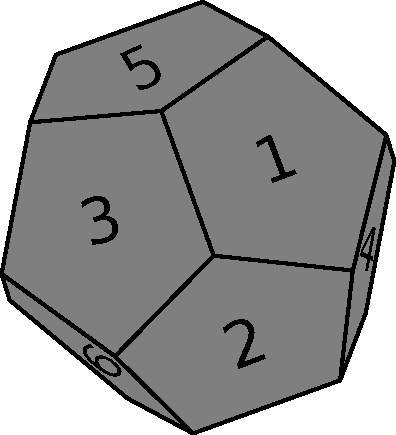
\includegraphics[width=1\linewidth]{sources/dice_rolls/images/3d_dices}
		\caption{Example of dice with $12$ faces.}
		\label{fig:dice_rolls:12faces_dice}
	 \end{subfigure}
	\hfill
	\begin{subfigure}[t]{0.25\textwidth}
		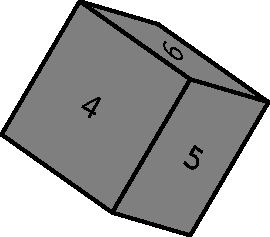
\includegraphics[width=1\linewidth]{sources/dice_rolls/images/cubic_dice}
		\caption{Example of common $6$ faces dice.}
		\label{fig:cycle_in_list:6faces_dice}
	 \end{subfigure}
	 \hfill
	 \begin{subfigure}[t]{0.25\textwidth}
		 \includegraphics[width=1\linewidth]{sources/dice_rolls/images/icosahedron_dice}
		 \caption{Example of dice with $20$ faces.}
		 \label{fig:cycle_in_list:20faces_dice}
	  \end{subfigure}
\end{figure}

\section{Discussion}
\label{dice_rolls:sec:discussion}

This is a classical Dynamic Programming problem that share lot of similarities with the \textit{Coin change} problem (See Chapter \ref{ch:coin_change}) to the point that you could solve this problem using the solution to the other. We can consider the problem in this chapter to be a specialization of the Coin change problem where the number of available coins is equal to $d$ and the denomination of the coins are $1,2,\ldots,f$.

I find very useful to start solving this problem in a brute-force \textbf{top-down} manner and then derive a faster version from it. 

\subsection{Brute-force}
\label{dice_rolls:sec:bruteforce}
The super easy brute-force solution in this case consist in finding all possible combinations and count the ones whose sum equals $t$. In this type of problem most of the time using recursion simplifies the implementation quite a bit. 
We start with the first dice and for this dice we have $f$ possible values we can assign to it, but once the value for this specific dice is set, let's say for the sake of this example $3$, then we are left with $d-1$ dices and we still have to make up for $t-3$  with those $d-1$ dices. So once a dice is rolled we are left with exactly the original problem on a smaller number of dices and target. This is why recursion is handy. This recursive process ends in two cases:

\begin{enumerate}
	\item $d<0$ or $t<0$ the answer is $0$. There is no solution to the problem when the number of dices to use is negative or the target number is negative.
	\item $t=0$. We have reached or target value. If we have used \textbf{all} dices then we have a solution otherwise not. So:
	\begin{itemize}
		\item if $d=0$, we have used all $d$ dices and the sum is exactly equal to $t$. This is a valid combination
		\item if $d>0$ then we have not set the value for all the dices and we have no more room for an additional value from another dice. This is not a good combination.
	\end{itemize}
\end{enumerate}


Listing \ref{list:dice_rolls:bruteforce} shows a possible implementation of such idea. Please note that this code is remarkably similar to the brute-force solution  for the Coin Change problem in Chapter \ref{ch:coin_change}.


\lstinputlisting[language=c++, caption={Brute-force (enumerating all possible combinations) solution for the problem of counting the number of dice rolls summing up to a target number $t$.},label=list:dice_rolls:bruteforce]{sources/dice_rolls/dice_rolls_solution1.cpp}

\subsection{Dynamic Programming - Recursive top-down}
\label{dice_rolls:sec:DP}

As per many other problems solvable with DP, the brute-force solution presented in Listing \ref{list:dice_rolls:bruteforce} can be turned into a much more efficient one by simply realizing that the same problem is solved over and over again. When this happens we can simply store the result of intermediate problems into a cache and use the values in the cache before trying to compute the answer (see Chapter \ref{valid_parenthesis:sec:dp}). 

For instance consider what happens during the execution of the code in Listing \ref{list:dice_rolls:bruteforce} for the following input:
\begin{itemize}
	\item $d = 3$
	\item $f = 6$
	\item $t = 12$
\end{itemize}

The function subproblem \inline{num_rolls_to_target_bruteforce(1,5,6)} solved $6$ times and the subproblem \inline{num_rolls_to_target_bruteforce(1,4,6)} is solved $5$ times. If you are not convinced draw the recursion tree, or add a print statement at the beginning of the function. All these superfluous execution can be avoided if the result of each of the subproblem is stored into a cache as shown in Listing \ref{list:dice_rolls:dp}. This implementation is an almost identical copy of the brute-force solution with the addition of a cache. Note how \textbf{before} actually trying to compute the answer we first look into the cache to see if we already did. If not, we solve the problem and before returning the answer we \textbf{save} the result into the cache.

\lstinputlisting[language=c++, caption={Dynamic programming with memoization top-down recursive  solution for the problem of counting the number of dice rolls summing up to a target number $t$.},label=list:dice_rolls:dp]{sources/dice_rolls/dice_rolls_solution2.cpp}


\section{Dynamic programming - Iterative bottom-up}
\label{dice_rolls:sec:bottom}

